\input ../SlidePreamble
\input ../preamble


\begin{document}

{\Huge

  \centerline{\bf TTIC 31230, Fundamentals of Deep Learning}
  \bigskip
  \centerline{David McAllester, Winter 2020}
  \vfill
  \vfil
  \centerline{Vector Quantized Variational Autoencoders (VQ-VAEs)}
  \vfill
  \vfill
  
\slide{Gaussian VAEs 2013}

\centerline{Sample {\color{red} $z \sim {\cal N}(0,I)$} and compute {\color{red} $y_\Phi(z)$}}

\vfill
\centerline{\includegraphics[width = 4in]{../images/VariationalFaces}}
\centerline{[Alec Radford]}

\slide{VQ-VAEs 2019}

\centerline{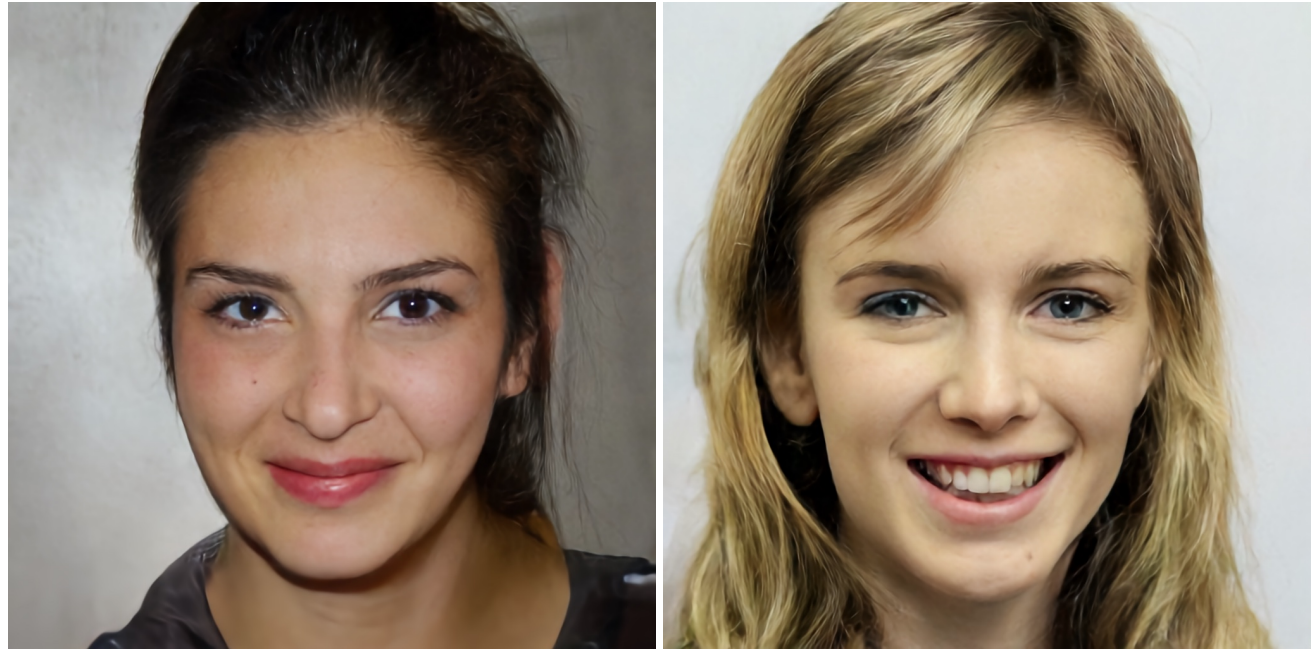
\includegraphics[width = 8in]{\images/VQ-VAE22}}

\vfill
VQ-VAE-2, Razavi et al. June, 2019

\slide{VQ-VAEs 2019}

\centerline{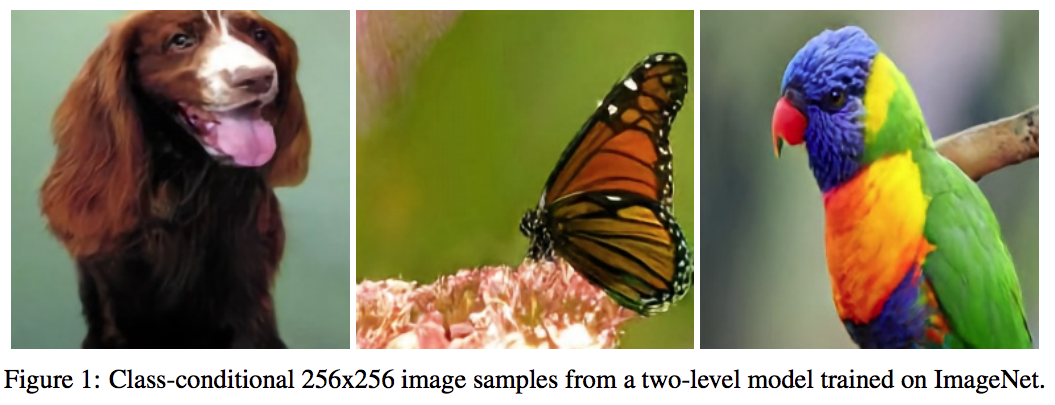
\includegraphics[width = 10in]{/users/davidmcallester/tex/images/VQ-VAE21}}

\vfill
VQ-VAE-2, Razavi et al. June, 2019


\slide{Vector Quantized VAEs (VQ-VAE)}

VQ-VAEs effectively perform $k$-means on vectors in the model so as to represent vectors by discrete cluster centers.

\vfill
For concreteness we will consider VQ-VAEs on images with a single layer of quantization.

\vfill
We use $x$ and $y$ for spatial image coordinates and use $s$ (for signal) to denote images.

\slide{VQ-VAE Encoder-Decoder}

We train a dictionary $C[K,I]$ where $C[k,I]$ is the center vector of cluster $k$.
\begin{eqnarray*}
L[X,Y,I] & = & \mathrm{Enc}_\Phi(s) \\
\\
z[x,y] & = & \argmin_k \;||L[x,y,I] - C[k,I]|| \\
\\
\hat{L}[x,y,I] & = & C[z[x,y],I] \\
\\
\hat{s} & = & \mathrm{Dec}_\Phi(\hat{L}[X,Y,I])
\end{eqnarray*}

\vfill
The ``symbolic image'' $z[X,Y]$ is the latent variable.

\slide{VQ-VAE as an RDA}

We will interpret the VQ-VAE as an RDA.

$$\Phi^*  =  \argmin_\Phi E_s\;I(s,z) + \lambda\mathrm{Dist}(s,\hat{s})$$

\vfill
The mutual information $I(s,z)$ is limited by the entropy of $z[X,Y]$ which can be no larger than $\ln K^{XY} = XY\ln K$.

\vfill
Maximizing $I(s,z)$ subject to this upper bound should reduce the distortion by providing the decoder with adequate information
about the image.

\slide{VQ-VAE Training Loss}

We preserve information about the image $s$ by minimizing the distortion between $L[X,Y,I]$ and its reconstruction $\hat{L}[X,Y,I]$.

\vfill
\begin{eqnarray*}
\Phi^* & = & \argmin_\Phi \;E_s\; \beta||L[X,Y,I] - \hat{L}[X,Y,I]||^2 + ||s -\hat{s}||^2
\end{eqnarray*}

\vfill
This is a two-level rate-distortion auto-encoder where the rate can be no larger than $XY\ln K$.

\slide{Parameter-Specific Learning Rates}

$$||L[X,Y,I] - \hat{L}[X,Y,I]||^2 = \sum_{x,y}\;||L[x,y,I] - C[z[x,y],I]||^2$$

\vfill
For the gradient of this they use

\begin{eqnarray*}
\mathrm{for}\;x,y\;\;L[x,y,I].\grad & \pluseq & 2\beta({L}[x,y,I]- C[z[x,y],I]) \\
\mathrm{for}\;x,y\;\;C[z[x,y],I].\grad & \pluseq & 2(C[z[x,y],I] - L[x,y,I])
\end{eqnarray*}

\vfill
This gives a parameter-specific learning rate for $C[K,I]$.

\vfill
Parameter-specific learning rates do not change the stationary points (the points where the gradients are zero).

\slide{The Relationship to $K$-means}

\begin{eqnarray*}
\mathrm{for}\;x,y\;\;C[z[x,y],I].\grad & \pluseq & 2(C[z[x,y],I] - L[x,y,I])
\end{eqnarray*}

\vfill
At a stationary point we get that $C[k,I]$ is the mean of the set of vectors $L[x,y,I]$ with $z[x,y] = k$ (as in $K$-means).

\slide{Straight Through Gradients}

The latent variables are discrete so some approximation to SGD must be used.

\vfill
They use ``straight-through'' gradients.

\begin{eqnarray*}
\mathrm{for}\;x,y\;\;L[x,y,I].\grad & \pluseq & \hat{L}[x,y,I].\grad
\end{eqnarray*}

\vfill
This assumes low distortion between $L[X,Y,I]$ and $\hat{L}[X,Y,I]$.

\slide{A Suggested Modification}

The parameter $\beta$ is paying two roles

\vfill
\begin{itemize}
\item It controls the relative weight of the two distortion losses.

\vfill
\item It controls the learning rate adjustment for the codebook.
\end{itemize}

\vfill
Shouldn't we have separate parameters for these two roles?

\slide{Training Phase II}

Once the model is trained we can sample images $s$ and compute the ``symbolic image'' $z[X,Y]$.

\vfill
Given samples of symbolic images $z[X,Y]$ we can learn an auto-regressive model of these symbolic images using a pixel-CNN.

\vfill
This yields a prior probability distribution $P_\Phi(z[X,Y])$ which provides a tighter upper bound on the rate.

\vfill
We can then measure compression and distortion for test images.  This is something GANs cannot do.

\slide{Multi-Layer Vector Quantized VAEs}
\centerline{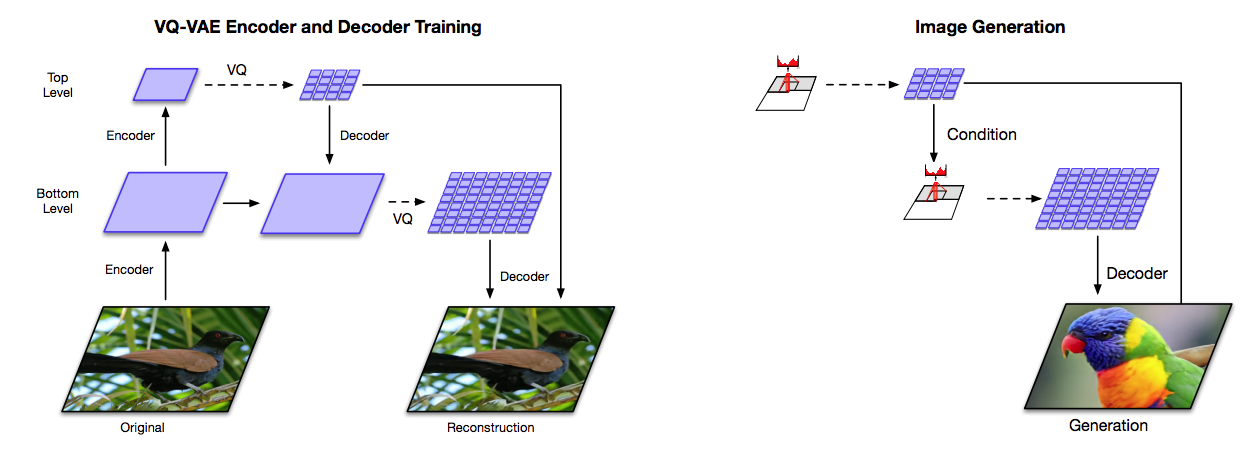
\includegraphics[width =10in]{\images/VQ-VAE24}}

\slide{Quantitative Evaluation}

The VQ-VAE2 paper reports a classification accuracy score (CAS) for class-conditional image generation.

\vfill
We generate image-class pairs from the generative model trained on the ImageNet training data.

\vfill
We then train an image classifier from the generated pairs and measure its accuracy on the ImageNet test set.

\vfill
\centerline{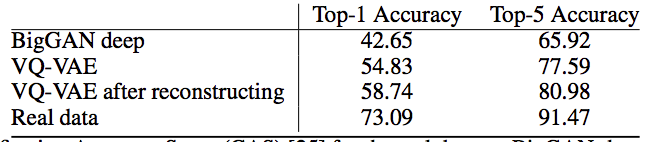
\includegraphics[width=7in]{\images/VQ-VAE23}}

\slide{Direct Rate-Distortion Evaluation.}

Rate-distortion metrics for image compression to discrete representations support unambiguous rate-distortion evaluation.

\vfill
Rate-distortion metrics also allow one to explore the rate-distortion trade-off.

\vfill
\centerline{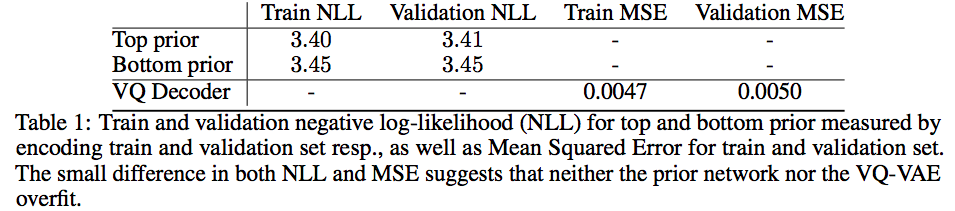
\includegraphics[width = 10in]{\images/VQVAE2Scores}}

\slide{Image Compression}

\vfill
\centerline{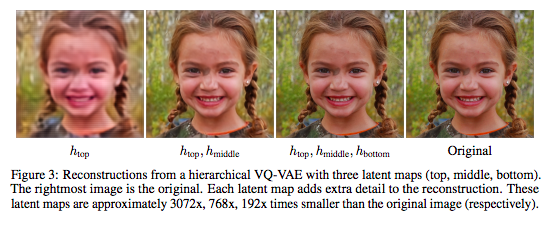
\includegraphics[width = 10in]{\images/VQgirl}}


\slide{Vector Quantization (Emergent Symbols)}

Vector quantization represents a distribution (or density) on vectors with a discrete set of embedded symbols.

\vfill
Vector quantization optimizes a rate-distortion tradeoff for vector compression.

\vfill
The VQ-VAE uses vector quantization to construct a discrete representation of images and hence a measurable image compression rate-distortion trade-off.

\slide{Symbols: A Better Learning Bias}

Do the objects of reality fall into categories?

\vfill
If so, shouldn't a learning architecture be designed to categorize?

\vfill
Whole image symbols would yield emergent whole image classification.

\slide{Symbols: Improved Interpretability}

Vector quantization shifts interpretation from linear threshold units to the emergent symbols.

\vfill
This seems related to the use of t-SNE as a tool in interpretation.


\slide{Symbols: Unifying Vision and Language}

Modern language models use word vectors.

\vfill
Word vectors are embedded symbols.

\vfill
Vector quantization also results in models based on embedded symbols.

\slide{Symbols: Addressing the ``Forgetting'' Problem}
When we learn to ski we do not forget how to ride a bicycle.

\vfill
However, when a model is trained on a first task, retraining on a second tasks degrades performance on the first (the model ``forgets'').

\vfill
But embedded symbols can be task specific.

\vfill
The embedding of a task-specific symbol will not change when training on a different task.


\slide{Symbols: Improved Transfer Learning.}

Embedded symbols can be domain specific.

\vfill
Separating domain-general parameters from domain-specific parameters may improve transfer between domains.

\slide{Unsupervised Machine Translation}

We can treat the German sentence $z$ as a latent variable in a probability model of a English sentence $y$.

$$\Phi^* = \argmin_\Phi\;E_{y,z \sim Q_\Phi(z|y)} \; \;-\beta \ln \frac{P_\Phi(z)}{Q_\Phi(z|y)} - \ln P_\Phi(y|z)$$

\vfill
Here $P_\Phi(z)$ can be a trained language model for German and $P_\Phi(y|z)$ and $Q_\Phi(z|y)$ are translation models.

\slide{Unsupervised Machine Translation}

In practice we use ``backtranslation''

$$\Phi^* = \argmin_\Phi\;\begin{array}{ll} & E_{y\sim \pop_y,\;z \sim Q_\Phi(z|y)} \; \;-\ln P_\Phi(y|z) \\ \\
+ & E_{z \sim \pop_z,\;y \sim P_\Phi(y|z)} \; \;-\ln Q_\Phi(z|y) \end{array}$$

\slide{END}

\end{document}
